\documentclass[pageno]{jpaper}

%replace XXX with the submission number you are given from the ASPLOS submission site.
\newcommand{\asplossubmissionnumber}{XXX}

\usepackage[normalem]{ulem}
\usepackage{xspace}
\usepackage{tabularx}

\usepackage{tikz}
\usepackage{tikzpeople}
\usetikzlibrary{shapes, shapes.misc}
\usetikzlibrary{arrows, arrows.meta, decorations.markings}
\usetikzlibrary{patterns}

\usepackage{algorithm}
\usepackage{algpseudocode}
\usepackage{amssymb}
\usepackage{algorithmicx}
%\algsetup{linenosize=\small}

\usepackage{graphicx}
\graphicspath{{figures/}}
%%%%%%%%%%%%%%%%%%%%%%%%%%%%
%     macro
% paper-specific definitions
\newcommand{\sys}[0]{Argus\xspace}
\newcommand{\xxx}[0]{Argus\xspace}
\newcommand{\nbug}[0]{11\xspace}
\newcommand{\mytitle}[0]{\textbf {Argus : Debugging Performance Issues in Modern Applications with Interactive Causal Tracing}}

% in short.
\newcommand{\eg}{{e.g.}}
\newcommand{\ie}{{i.e.}}
\newcommand{\etc}{{etc}}
\newcommand{\para}[1]{\vspace{.00in}\noindent{\bf #1}}
\newcommand{\wrt}{{w.r.t. }}
\newcommand{\cf}{{cf. }}
\newcommand{\etal}{{et al. }}
\newcommand{\vv}[1]{{\texttt{#1}}}

%for algorithm
\algnewcommand\algorithmicswitch{\textbf{switch}}
\algnewcommand\algorithmiccase{\textbf{case}}
\algnewcommand\algorithmicassert{\texttt{assert}}
\algnewcommand\Assert[1]{\State \algorithmicassert(#1)}%
% New "environments"
\algdef{SE}[SWITCH]{Switch}{EndSwitch}[1]{\algorithmicswitch\ #1\ \algorithmicdo}{\algorithmicend\ \algorithmicswitch}%
\algdef{SE}[CASE]{Case}{EndCase}[1]{\algorithmiccase\ #1}{\algorithmicend\ \algorithmiccase}%
\algtext*{EndSwitch}%
\algtext*{EndCase}%
\let\oldemptyset\emptyset
\let\emptyset\varnothing
\makeatletter
\algrenewcommand\ALG@beginalgorithmic{\footnotesize}
\makeatother

\begin{document}
\title{\mytitle}

\date{}
\maketitle

\thispagestyle{empty}
\begin{abstract}
MacOS is well known for its friendly user experience.
However, performance bugs still exists, which annoys users.
For instance, spinning cursors are threw out from time to time.
Although the reason why it appears is straightforward based on its mechanism that the main UI thread is too busy to process user input, its root cause is still hard to diagnose.
%dependancy graph is useful to diagnose performance bugs
Tracking the performance bug where the lagging or unresponsiveness of applications stem, is hard due to the massive interactions among threads.
Without instruments in the source code, it is challenging to detangle the user transactions running concurrently in the system, as well as the background heartbeat threads.
\par
Fortunately, instruments in low level libraries and system could help developers to recognize interations of threads,
by generating a dependancy graph over the tracing data.
A tracing point, the statement where the instrument resides, contains the name of an event and attributes correlated to the event. 
Each of them either represents the execution boundary of a particular request/user input or reflects the potential connections with other events. 
With events inside the boundary of particular request/user input as node, and connections as edges, a dependancy graph can be generated for each user transaction.
The dynamically generated dependancy graph is useful, in that it helps developers to figure out the critial path of user transations and enlight them to improve their code.
%short-commings of dynamic generated dependancy graph
\par
However, without the in-depth understanding of a system, especially when it is not open source, the integrity and completeness of the generated dependancy graph is hard to gurantee.
The incorrect graph becomes less useful, event misleading, for the developers to figure out the root cause of performance bugs.
%how to address
In this paper, we focus on Apple's Mac system and address the challenges by inspecting the over connections and under connections in the dependancy graph, which is generated with well-known programing paradigms.
Revealing the problematic edges or nodes caused by specific programming paradigms provides hints to the developers.
With these hints, the developers can further explore pragraming paradigms in various levels, including kernel, dynamic libraies and middle-ware frameworks.
As a result, the dependancy graph gets improved cumulatively and becomes more helpful to figure out the root cause of the performance bugs.

\end{abstract}
\section{Introduction} \label{sec:intro}
Today's web and desktop applications are predominantly parallel or distributed,
making performance issues in them extremely difficult to diagnose because the
handling of an external request is often spread across many threads, processes,
and asynchronous contexts instead of in one sequential execution
segment~\cite{harter2012file}.  To manually reconstruct this graph of execution
segments for debugging, developers have to sift through a massive amount of log
entries and potentially code of related application
components~\cite{chen2002pinpoint, zhao2016non, xu2009detecting,
nagaraj2012structured, yuan2012conservative}.  More often than not, developers
give up and resort to guessing the root cause, producing ``fixes'' that
sometimes make the matter worse.  For instance, a bug in the Chrome browser
engine causes a spinning cursor in MacOS when a user switches the input
method~\cite{chromiumbugreport}.  It was first reported in 2012, and developers
attempted to add timeouts to work around the issue.  Unfortunately, the bug has
remained open for seven years and the timeouts obscured diagnosis further.

Prior work proposed \emph{Causal tracing}, a powerful technique to construct
request graphs (semi-)automatically~\cite{zhang2013panappticon}. It does so by
inferring (1) the beginning and ending boundaries of the execution segments
(vertices in the graph) involved in handling a request; and (2) the causality
between the segments (edges)---how a segment causes others to do additional
handling of the request.  Prior causal tracing systems all assumed certain
programming idioms to automate inference.  For instance, if a segment sends a
message, signals a condition variable, or posts a task to a work queue, it
wakes up additional execution segments, and prior systems assume that wake-ups
reflect causality.  Similarly, they assume that the execution segment from the
beginning of a callback invocation to the end is entirely for handling the
request that causes the callback to be
installed~\cite{zhang2013panappticon, ravindranath2012appinsight}.
Causal tracing is quite effective at aiding developers to understand complex
application behaviors and debug real-world performance issues.% in XXX.

Unfortunately, based on our own study and experience of building a causal
tracing system for the commercial operating system MacOS, we found that modern
applications frequently violate these assumptions. Hence, the request graphs
computed by causal tracing are imprecise in several ways.  First, an inferred
segment may be larger than the actual event handling segment due to batch
processing.  Specifically, for performance, an application or its underlying
frameworks may bundle together work on behalf of multiple requests with no
clear distinguishing boundaries.  For instance, WindowServer in MacOS sends a
reply for a previous request and receives a message for the current request
using one system call mach\_msg\_overwrite\_trap, presumably to reduce
user-kernel crossings.

Second, the graphs may be missing numerous causal edges.  For instance,
consider ad hoc synchronization~\cite{xiong2010ad} via shared-memory flags: a
thread may set ``\vv{flag = 1}'' and wake up another thread waiting on
``\vv{while(!flag);}'' to do additional work.  Even within one thread, the code
may set a data variable derived from one request and later uses it in another
request (\eg, the buffer that hold the reply in the preceding WindowServer
example). Although the number of these flags may be small, they often express
critical causality, and not tracing them would lead to many missing edges in
the request graph.  However, without knowing where the flags reside in memory,
a tool would have to trace all memory operations, incurring prohibitive
overhead and adding many superfluous edges to the request graph.

Third, in any case, many inferred edges may be superfluous because wake-ups do
not necessarily reflect causality.  Consider an \vv{unlock()} operation waking
up an thread waiting in \vv{lock()}.  This wake-up may be just a happens-stance
and the developer intent is only mutual exclusion.  However, the actual
semantics of the code may also enforce a causal order between the two
operations.

We believe that, without detailed understanding of application semantics,
request graphs computed by causal tracing are \emph{inherently} imprecise and
both over- and under-approximate reality.  Although developer annotations can
help improve precision~\cite{barham2004using, reynolds2006pip}, modern
applications use more and more third-party libraries whose source code is not
available.  In the case of tech-savvy users debugging performance issues such
as a spinning (busy) mouse cursor on her own laptop, the application's code is
often not available.  Given the frequent use of custom synchronizations, work
queues, and data flags in modern applications, it is hopeless to count on
manual annotations to ensure precise capture of request graphs.

In this work, we present \xxx, a practical system for effectively debugging
performance issues in modern desktop applications despite the imprecision of
causal tracing.  \xxx's goal is not to construct a per-request causal graph
which requires extremely precise causal tracing.  Instead, it captures an
approximate event graph for a duration of the system execution to aid
diagnosis.  We designed \xxx to be interactive, as a debugger should rightly
be, so that its users can easily inspect current diagnostics and guide the next
steps of debugging to counter the inherent imprecision of causal tracing. For
instance, \xxx's event graph contains many inaccurate edges that represent
false dependencies, which the user can address in an interactive manner.  When
debugging a performance issue using \xxx, a user need only make edges relevant
to the issue precise.  In other words, she can provide schematic information on
demand, as opposed to full manual schema upfront for all involved applications
and daemons~\cite{barham2004using}.

Moreover, \xxx enables users to dynamically control the granularity of tracing
using a number of intuitive primitives. The system begins by using always-on,
lightweight, system-wide tracing.  When a user observes a performance issue
(\eg, a spinning cursor), she can inspect the current graph \xxx computes,
configure \xxx to perform finer-grained tracing (\eg, logging call stacks and
instruction streams) for events she deems relevant, and trigger the issue again
to construct a more detailed graph for diagnosis.  \xxx also supports
interactive search over the event graphs that contain both normal and buggy
executions for diagnosis.

We implemented \xxx in MacOS, a widely used commercial operating system. MacOS
is closed-source, as are its common frameworks and many of its applications.
This environment therefore provides a true test of \xxx.  We address multiple
nuances of MacOS that complicate causal tracing, and built a system-wide,
low-overhead tracer.

We evaluated \xxx on \nbug real-world, open spinning-cursor issues in widely
used applications such as the Chromium browser engine and MacOS System
Preferences, Installer, and Notes.  The root causes of all \nbug issues were
previously unknown to us and, to a large extent, the public. Our results show
that \xxx is effective: it helped us find all root causes of issues, including
the Chromium issue that remained open for seven years.  \xxx is also fast: its
systems-wide tracing incurs only 1\% CPU overhead overall.

This paper makes the following contributions: our conceptual realization that
causal tracing is inherently imprecise and that interactive causal tracing is
superior than prior work in debugging performance issues in modern
applications; our system \xxx that performs system-wide tracing in MacOS with
little overhead; and our results diagnosing real-world spinning (busy) cursors
and finding root causes for performance issues that have remained open for
seven years.

This paper is organized as follows. In Section~\ref{sec:overview}, we present
an overview of using \xxx and a Chromium example.
Section~\ref{sec:dependency-semantics} describes our approach to identifying
semantic dependencies, and Section~\ref{sec:implementation} describes our
tracing implementation. In Section~\ref{sec:casestudy} we present other case
studies, and Section~\ref{sec:evaluation} contains our performance evaluation.
We summarize related work in Section~\ref{sec:related-work}, and end with
conclusion in Section ~\ref{sec:conclusion}.

\section{Overview} \label{sec:overview}

\subsection{\xxx Work Flow}

\begin{figure*}[tb]
    \centering
    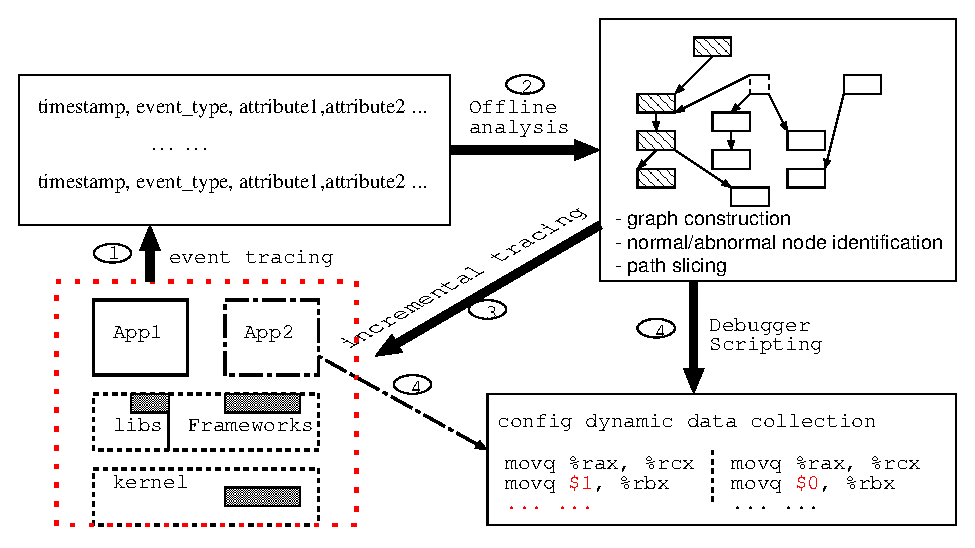
\includegraphics[width=0.8\linewidth]{ArgusOverview.eps}
    \caption{\xxx Work Flow}
    \label{fig:argus-overview}
\end{figure*}

Figure~\ref{fig:argus-overview} shows \xxx's work flow, which consists of
two phases.  A user runs command ``\v{\xxx start}'' to
enter the system-wide tracing phase, within which \xxx logs events
including system calls, inter-process communications (IPCs), and waits and
wake-ups from all applications and daemons.  Occasionally based on user
configurations, it logs data flag accesses leveraging hardware
watch-point registers.  Each log entry includes a timestamp, the event
type, key attributes of the event, and a lightweight call stack obtained
by unwinding the stack pointer.  \xxx implements tracing by instrumenting
core system libraries and a small portion of the operating system.  The
performance impact of this system-wide tracing is low because the logged
events themselves are often expensive and require user-kernel crossings,
masking the overhead of tracing.

Whenever a user detects a performance issue such as a spinning cursor, she
runs ``\v{\xxx debug}'' to enter the interactive diagnosis phase.  \xxx
initializes this phase by constructing a causal graph from all logged
events up to user-specified duration.  Rather than requiring a precise
application-specific user-written schema, \xxx leverages a simple
system-wide schema we created to construct approximate graphs
(\S\ref{subsec:graph}), and relies on interactive user insights for
diagnosis (\S\ref{subsec:debug}).

\subsubsection{Constructing Event Graphs} \label{subsec:graph}

\xxx defines the beginning of an execution segment as one of the following
three types of events (1) the beginning of a thread, (2) the event from a
wait operation such as \v{pthread\_cond\_wait()} or
\v{mach\_msg\_receive()}, and (3) the first logged event of a thread
because tracing may start mid execution.  It similarly defines the end of
an execution segment as (1) the exit of a thread, (2) the call to a wait
operation, and (3) the last logged event of a thread.

\xxx defines the edges as follows.  First, the return from a wait
operation causally depends on the wake-up operation.  Since an application
or its libraries may define custom synchronization primitives, \xxx traces
wait and wake-up operations inside the operating system kernel (the
\v{waitq\_assert\_wait64\_locked} \and \v{thread\_unblock} functions in MacOS kernel).
This design decision ensures that \xxx captures a large set of casual
edges at the expense of superfluous edges that do not map to causality.
For instance, inside a system call or interrupt handler, the kernel
typically checks whether the current process has used up its time slice
and, if so, wakes up another process.  \xxx thus explicitly filters out
edges due to kernel maintenance (in \v{interrupt()} and
\v{sched\_timeshare\_miantenance\_continue} in MacOS) instead of application intent.
Second, the read of a data flag causally depends on the write of the
same flag.  Edges of this type are few but critical for diagnosis.  Third,
the timer expiration and cancellation events causally depend on the
installation of the timer.  Fourth, each execution segment has an incoming
edge from the immediately preceding segment in the same thread.  \xxx
considers this type of intra-thread edges weaker than inter-thread edges
due to the wait between the two segments.  In its analysis, \xxx follows
intra-thread edges typically only when it cannot find any inter-thread
edges.

It is easy for a user to incrementally extend \xxx with custom segment
boundaries and edges.  For instance, to handle batch processing, we
created a heuristic that splits a segment if it has outgoing edges to two
or more different processes (unless the attributes of the corresponding
events indicate otherwise).  We also added edges for three data flags and
8 custom communication primitives (see \S\ref{subsec:tcp}).

\subsubsection{Interactive Diagnosis} \label{subsec:debug}

After \xxx builds the event graph, a user can interactively query this
graph for diagnosis.  For instance, consider a spinning cursor in MacOS
which indicates the current application's main thread has not processed
any UI events for over two seconds.  The user can query \xxx to find the
ongoing event in the application's main thread concurrent to the display
of the spinning cursor.  Depending on the type of the event, she can
proceed in three directions.

First, if the concurrent event is a busy operation that occupies the CPU,
she has found the cause of the spinning because a busy main thread cannot
process UI events.  She can examine the event's lightweight call stack.
If it does not provide enough details, she can rerun the application and
use \xxx's fine-grained debugging tool to obtain a more complete call
stack, the addresses of the instructions executed, and parameters and
return values of call instructions.  In general, she can increase
debugging details for any event, not just a busy event.

Second, if the concurrent event is a blocking wait, she runs \xxx to
locate another event in the graph that causes the wake-up to arrive
late. \xxx does so using the following idea.  In the normal case, there
must be a path of wake-up edges that leads to the blocking wait, so the
main thread starts running again.  In the spinning case, somewhere along
the path, a thread's wake-up is missing, so this thread is the culprit.
Mechanically, \xxx first searches the graph to find a similar wait that
does not cause a spinning cursor.  If there are multiple nodes similar to
the wait, \xxx asks the user to pick one.  It then slices the graph
backwards to find the wake-up path.  If an event has exactly one
inter-thread edge or only an intra-thread edge, it follows the edge.
Otherwise, the event must have two or more inter-thread edges, and \xxx
consults the user to pick one to follow.  Given the path, \xxx examples
the threads in the path one by one, and returns the thread whose wake-up
is missing in the spinning case.

Third, if the concurrent event is a thread yield, it is highly indicative
that the main thread is waiting on a data flag (\eg, ``while(!done)
thread\_switch();'').  To discover a data flag, the user reruns the
application with \xxx to collect instruction traces of the concurrent
event in both the normal and spinning cases and detects where the control
flow diverges.  She then reruns the application with \xxx to collect
register values for the basic blocks before the divergence and uncovers
the address of the data flag.  She then configures \xxx to log accesses to
the flag during system-wide tracing.

The user can recursively apply \xxx to further diagnose ``the culprit of
the culprit.''  For instance, 

Based on our results, the first type of spinning cursor is more common but
the second and third types cause the most harm.  The reason is that the
first type tends to be straightforward to diagnose, so they are fixed
quickly.  The second and third types involve multiple threads, so they are
extremely hard to understand and fix even for the application's own
developers.  Therefore, they remain open for years and ruin many users'
experiences.

\subsection{Chromium Spinning Cursor Example}

%   resolve symbol, save to log
%     search for set\_spinning
%     if found,
%       find main thread node at the time of set\_spinning
%     find fontd
%     manually check nodes in each thread immediately after the nodes in the slice (normal abnormal boundary)
%  output is a node, and a HTML dump of node and immediate predecessors and successors
% systems preference          
%  spinning node in UI thread is not waiting
%  so we look for messages, and find the diff

One of the authors experienced first-hand the aforementioned performance
issue in Chromium, an open-source browser engine that powers Google Chrome
and, starting recently, Microsoft Edge~\cite{chromiumurl}.  She tried to type in
the Chromium search box a Chinese word using SCIM, the default Chinese
Input Method Editor that ships with MacOS.  The browser appeared frozen
and the spinning cursor occurs for a few seconds.  Afterwards everything
went back to normal.  This issue is reproducible and always ruins her
experience, but it is quite challenging to diagnose because two
applications Chromium and SCIM and many daemons ran and exchanged
messages.  This issue was reported by other users for other non-English
input methods, too.

To diagnose this issue with \xxx, the author started system-wide tracing,
typed an English string in the search box first to get the events in a
normal case, and then reproduced the spinning cursor with a Chinese search
string typed via SCIM.  The entire session took roughly five minutes.

She then ran \xxx to construct the event graph.  The graph had 2,749,628
vertexes and 3,606,657 edges, almost fully connected.  It spans across 17
applications; 109 daemons including \v{fontd}, \v{mdworker}, \v{nsurlsessiond}
and helper tools by applications; 126 processes; 679 threads, and 829,287 IPC
messages.  Given the scale of the graph and the diverse communication patterns,
it would be extremely challenging for prior automated causal tracing
tools~\cite{aguilera2003performance}, \cite{zhang2013panappticon},
\cite{attariyan2012x}, \cite{cohen2004correlating} because they handle a fairly
limited set of patterns.  Tools that require manual
schema~\cite{barham2004using} \cite{reynolds2006pip}, would be prohibitive
because developers would have to provide schema for all involved applications
and daemons.

\begin{figure*}[tb]
    \centering
    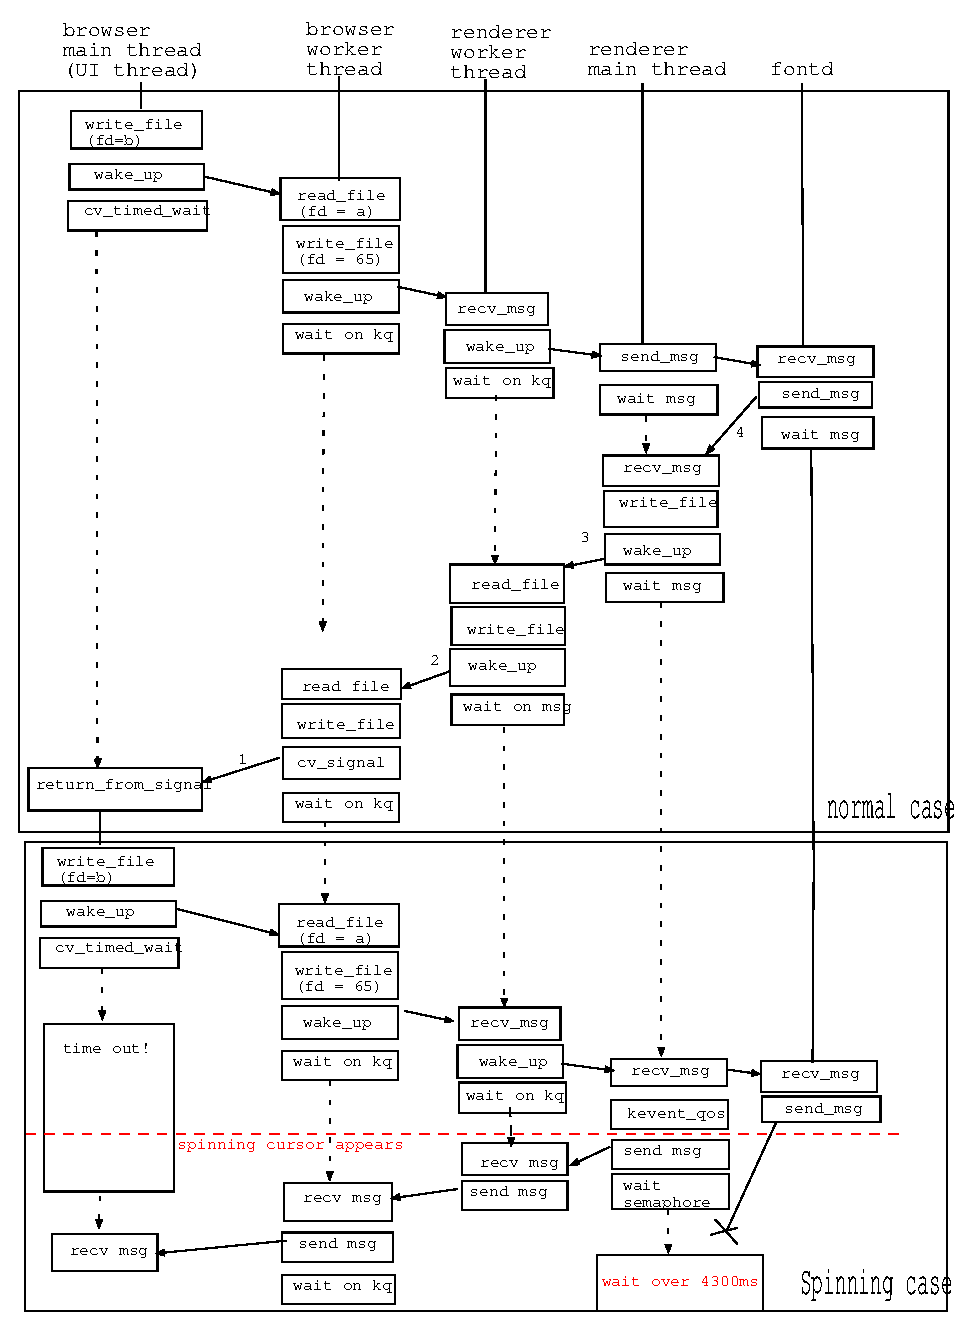
\includegraphics[width=0.8\linewidth]{chromium_case_study.eps}
    \caption{Chromium case study.}
    \label{fig:chromium-trace}
\end{figure*}

Next she ran \xxx to find the event in the main thread of the browser
process.  \xxx returned a \v{cv\_timed\_wait} event
(Figure~\ref{fig:chromium-trace}) that blocked the main thread for a few
seconds.  Inspection of the lightweight call stack reveled that this wait
happened within a call to \v{TextInputClientMac::GetFirstRectForRange}.
Without knowing the application's semantics, she could not understand this
method.  Thus she ran \xxx to compare the spinning case to a normal case.
\xxx searched in the main thread of the browser process for vertexes
similar to this wait waiting vertexes similar to this wait, found three,
and confirmed with the user which one she wanted.

\xxx then found the normal-case wake-up path shown in the figure, which
connects five threads.  The browser main thread was signaled by a browser
worker thread as shown in step \textcircled{1} of backward slicing in Figure
\ref{fig:chromium-trace}, which in turn wake up for \v{read\_file} in step
\textcircled{2} for IPC from a worker thread of \v{renderer}, the daemon for
rendering screens.  The \v{renderer} worker thread is woken up by the
\v{renderer} main thread to \v{read\_file} as \textcircled{3} in the backward
slicing, which in turn \v{recv\_msg} \textcircled{4} from \v{fontd}, the font
service daemon.  From this path, we could guess that \v{GetFirstRectForRange}
was for the browser to understand the bounding box of the search string.  \xxx
further compared the wake-up path with the spinning case, and returned the
\v{wait\_semaphore} event in the \v{renderer} main thread, the culprit that
delayed waking up the browser main thread over 4 seconds.

What caused the wait in the \v{renderer} main thread though?  She thus
continued diagnosis and recursively applied \xxx to the wait in
\v{renderer}, and got the wake-up path shown in the figure for this wait.
Inspection revel that the \v{renderer} requested the browser's help to
render Javascript and was waiting for a reply.  At this point, a circular
wait formed because the browser was waiting for the \v{renderer} to return
the string bounding box and the \v{renderer} was waiting for the browser
to help render Javascript.  This circular wait was broken by a timeout in
the browser main thread (the \v{cv\_timed\_wait} timeout was
1,500 ms).  While the system was able to make progress, the next key press
caused the spinning cursor to display for another 1,500 ms.  The timeout
essentially converted a deadlock into a livelock.

\subsection{Limitations}

\xxx is designed to support interactive debugging of performance issues.
To incrementally obtain more fine-grained event traces, it needs to rerun
an application to reproduce a performance issue.  Thus, if the issue is
difficult to reproduce, we have to rely on the log collected by the
lightweight system-wide tracing for debugging, and lose the benefits of
interactivity.  Fortunately, a performance issue that almost never
reproduces is probably not as annoying as one that occurs frequently.

We implemented \xxx in the closed-source MacOS which presents a harsh test
for \xxx, but we have not ported \xxx to other operating systems yet.  It
is possible that the ideas and techniques do not generalize to other
operating systems.  However, modern operating systems share many
similarities, and good ideas tend to flow both ways, so we are hopeful
that the ideas in \xxx are generally applicable.  Similarly, the
applications and performance issues used in our evaluation may be
non-representative.

\subsubsection{Argus Graph Computing}
\begin{itemize}
\item \xxx constructs dependency graphs with the events from tracing logs. The graphs are equivalent to a high level control flow graphs.
%%Events traced by \xxx can be classified into three categories based on purposes: preserve higher level semantics, construct connections across inter and itra thread boundaries, define boundaries for batch processing within a thread. A vertex contains a list of events constrainted by intra-thread boundaries. Its semantics relies on the semantics events from the list. Edges across the threads usually indicated the two threads are working on behalf of the same task.
\item As noticed that not all wake-up edges stands for a causality, \xxx applies default hueristicsto filter out definitive noises: interrupt/kernel maintainance/timer expirations
\item The graph is inherently inaccurate given the existance of spurious edges. (mutex lock example)
\item Despite of the inaccurary, the graph with the causality edges is still helpful in debugging complicated performance bugs, which involve mutilple processes and threads.
\end{itemize}

\subsubsection{User Interactions}
\begin{itemize}
\item Making the graph sound without user interaction is almost impossible given essential attribite of commericial operating system as a grey box.
\item Over connections occur if intra-thread boundaries are missing from batch processing programming paradigms. (dispatch\_mig\_service, runloop)
\item Data dependencies inter/intra threads are usually hard to fully exploit in the initial pass of graph computing. (shared flags in Object, data dependency for delay work intra-thread)
\end{itemize}

%%\section{Patterns}

We encountered several instances of runtime event dependencies between thread
contexts. We present several generalizable cases below.

\para{Signal handling}
Sometimes, a signal handler happens to run within a thread's context, for
example, a timer interrupt. We identify the start and end of the
signal-handling code to splice it away from the containing context, since it is
usually unrelated.

\begin{verbatim}
thread 1      thread 2

sleep(50);    running
              process receives timer interrupt();
                signal_handler
                  make_runnable(thread_1);
\end{verbatim}

\para{Kernel takes over context}
As part of a thread context switch, an execution context may enter kernel
space. The code will enter kernel scheduling and wake up another
\texttt{kernel\_task} thread.

\begin{verbatim}
thread_invoke(self, new_thread) // thread switch, kernel space
  sched_timehsare_consider_maintance()
    wake up another kernel_task thread
\end{verbatim}

To detect this case, we filter wakeups from the kernel timer, interrupt
handler, or kernel shared memory maintenance. Such cases represent spurious
dependencies. However, sometimes when a worker thread wakes up another worker
thread, this can represent a true dependency. The distinguishing feature is
whether a synchronization primitive (shared memory) is used.

\para{Batching in event processing}
The WindowServer MacOS system daemon contains an event loop which waits on Mach
messages. Conceptually, it processes a series of independent events from
different processes. However, to save on kernel boundary crossings, it uses a
single system call to receive data and send data for an unrelated event. This
batch processing artificially makes many events appear dependent, and we split
the execution segments to maintain the independence of the events.

\begin{verbatim}
  while() {
    message = receive and send Mach msg(pending_reply) // reduces
kernel crossing presumably
    process message
    if (message needs reply)
      pending_reply = reply // only keeps one pending message
  }
\end{verbatim}

\para{CoreAnimation shared memory}
CoreAnimation contains a worker thread which sets a global variable inside
animation objects whenever the object needs to be repainted. The main thread
iterates over all animation objects and reads this flag, rendering any such
object. This creates a dependency between the main thread and CoreAnimation,
but these dependencies are extremely common and do not communicate much
information.

\begin{verbatim}
  worker thread that needs to update UI
  ObjCoreAnimation->need_display = 1

  main thread:
  traverse all CoreAnimationobjects
  if obj->need_display == 1
    render(obj)
\end{verbatim}

\para{Spinning beach ball shared flag}
Whenever the system determines that the main thread has hung for a certain period, and the spinning beach ball should be displayed, a shared memory flag is set. Access to this flag is controlled via a lock, i.e. the lock is used for mutual exclusion, and does not imply a happens before relationship.

\begin{verbatim}
  NSEvent thread                      main thread

while()
  NSArray[produced++] = event
  event_dispatched = 1
  if main_thread_spinning != 1n
    register_timer(2 seconds, callback_closure}
                                    while()
                                      event = NSArray[consumed++];
      process event;
    callback_closure
      if event_dispatched == 1
        main_thread_spinning = 1
                                      if main_thread_spinning == 1
      main_thread_spinning = 0;
              event_dispatched = 0
\end{verbatim}

\para{Dispatch message batching}
The message dispatch service dequeues messages from many processes and staggers
processing of the messages. This creates false dependencies between each
message in the dispatch queue.
\begin{verbatim}
fontd

worker thread

dispatch_queue.enqueue(
   your code
)
  // create block function


block = dispatch_equeue.dequeue()
block
  dispatch_mig_service()
    while(){
      receive mach message
      process
      optional reply if needed
    }
\end{verbatim}

\para{Mach message mismatch}
Use recv port to connect messages.

\begin{verbatim}
thread 1,proc1      thread 2,proc2    thread 3,proc2    thread 4, proc 1
send mach msg1
                  recv mach msg1
      send mach msg2
                                      recv msg2
              send msg3
                            recv msg3 // reply
 xpc (higher than mach msg
 scim to chrome

 scrim thread   t2          chrome worker thread            chrome main thread
  send (msg has recv port)
                           dispatch_mach_msg_recv
                                        ?

xpc_connection_and_send_msg (msg has scim recv port)
               recv
\end{verbatim}

\para{Runloop callbacks}
As is common in event driven programming, many methods can post a callback to a runloop to continue processing at a later time.

\begin{verbatim}
done by another thread
callout_to_runloop(runloop, source, port, cb) cb installation
log runloop, source, port, cb // runloop, source, port help identify
the right execution of cb() to connect to

   runloop will call cb()
   cb begin: we log runloop, source, port so right match
\end{verbatim}


\para{Timers}
Most timers in MacOS are repeat timers, meaning that the timer reregisters itself before finishing.
This creates complex dependencies because timers are invoked asyncronously during interrupts.


\begin{verbatim}
\
timer_create
     |       \ (may or may not fire)
     |        timer_expire
     |
timer_cancel
     |
timer_create
     |
timer_create  // repeat timer?
            \timer_expire

\end{verbatim}

add instrumentation after every occurrence of instruction seq: also supply c function to log

\section{Implementation}
We now discuss how we collect tracing events from both kernel and libraries.

\subsection{Instrumentation}
Like Detour~\cite{detourXXXXXXXX}, we use static analysis to decide which instrumentation to perform, and then enact this instrumentation at runtime. 
On MacOS, most libraries as well as many of the applications used day-to-day are closed-source.
Adding tracing points to such code requires binary instrumentation.
Techniques such as library preloading to override individual functions are not applicable on MacOS, as libraries use two-level executable namespaces.
Hence, we implemented a binary instrumentation mechanism that allows developers to add tracing at any location in a binary image.

XXX I thought a user can specify a search sequence of instructions, and our system adds instrumentation when the sequence is found in binary.  If so we want to emphasize it a bit as this feature is different from detour.
XXX say that instrumentation code is written in C

To add instrumentation, we insert 5-byte call instructions into the program. The user finds a location of interest in the code related to a specific event,
and we overwrite the victim instructions at that location. We create a new trampoline target function, whose first few instructions are those which were overwritten.
All of the trampoline functions are grouped together by our tool and a new library is generated.
This library provides the same public API as the original and is a drop-in replacement. We load and call the original code as an unmodified shared library.
The detours or trampoline calls are added by an initialization function in our new library; we temporarily mark the code region as writable with \texttt{mprotect}
to calculate offsets and perform the modifications. The initialization is called externally through \texttt{dispatch\_once}.
To use the modified libraries, we simply replace system libraries in their original locations (renaming them so that our code can access the originals).

One potential issue is that we use 5-byte call instructions with 32-bit displacements to jump from the original library to our new one.
This design requires that the libraries be loaded within +/- 2GB of each other in the 64-bit process address space.
However, since we list each original library as a dependency of our new libraries, the system loader will map each new and original library in sequence.
In practice, the libraries ended up very close to one another and we did not see the need to implement a more general long-jump mechanism.

\subsection{Tracing Events}
Current MacOS systems support a system-wide tracing infrastructure built by Apple. [traces what]
By default, the infrastructure temporarily stores events in memory and flushes them to screen or disk when an internal buffer is filled.
We extended this infrastructure to support larger-scale tests without filling up the disk by implementing a ring buffer backed by a file.
We store at most 2GB of data [per log?], which corresponds to approximately XXX events (XXX time).

\subsection{Tracing Custom Primitives}
The graph should be incrementally improved with new tracing points.
The procedure to discover such programming paradigm can be repeated on regular executions before tracing for diagnosis.
The missing connections are much harder to explore.
As long as the remaining connections in the current graph help diagnosis, it is not necessary to explore.

\xxx provides two lightweight tools for users to collecting data with incremental tracing, instead of the lldb.
\begin {itemize}
\item For any given shared variable of interest, we take advantage of hardware watchpoints.
	Tracing points are recorded in the watchpoint handler when the variable is accessed.
	We hook the handler in CoreFoundation to make sure that it is loaded correctly into the address space of our target application.
	We set the hardware watchpoint in an ad-hoc manner with a custom command-line tool.
\item For any code location where user want to check its call stacks, our interface accepts a tag as input to distiguish.
	It unwindes the rbp from the user stack to store the valid return addresses in the buffer. The buffer is recorded into the log as tracing events.
	These address woulg go through the offline symbolicator in the graph construction phase.
\end{itemize}

XXX give a simple command line example of how a user can ask \xxx to trace a data flag
XXX say what we do in watch point exception handler (record instruction so can determine read or write, and reg values)

In \xxx, we patched the kernel with 1193 lines of code,
and we instrumented the libraries including: libsystem\_kernel.dylib, libdispatch.dylib, libpthread.dylib, CoreFoundation, CoreGraphics, HIToolbox, AppKit and QuartzCore with our binary instrumentation libraries. 
Based on the new libraries creatd, the user can easily add tracing points with exposed API and the usage sample inside.

\subsection{Capturing Instructions for Diagnosis}

XXX Talk about what data we gather using lldb, the debugger in the LLVM compiler tool chain.

After the offline analysis on the graph, we take the API covers the fine range as input to our debugging scripts.
The debugging scripts go throught the instruction from application and higher level frameworks step by step.
The purpose is to capture the parameters results from the user interaction.
Once a new function begins by checking the instruction, we record the call stacks for comprehension. 
For API from the low level libraries, such as pthread, we step over and record the return value.
AS the operation are confined in the small range, the overhead is not too much.

Both the execution on normal case and problematic case are recorded, our tool further compares the log and report
the difference, with the full call stack.

\subsection{Finding Similar Events}

The performance isssue caused by the busy processing in UI thread is quite straightforward to diagnoze with out tool.
Debugging the UI thread blocking on the contention of resource is much more difficult.
In this situation, our tool is required to recognize the corresponding node
which obtained the resource in its normal execution.

Node comparision algorithm helps to allieviate users from the burden of inspecting large logs.
We first normalize the nodes with selected events.
In our system, we exclude the interrupts from the comparison
since the number and type of interrupts are usually different from execution to exection.
For the events that connected to other events, we normalize it with a peer attribute
to record the process id of its connecting peer,
We also record the name of the system calls, message id carried in mach\_msg for corresponding events.
The comparison algorithm omits the repeating times of the same events,
by checking if one node contains all distinct events in the other node.

The above step only idenfity the similarity of nodes.
We also define the differential attribtes to distinguish the normal node and spinning node,
including the waiting time, execution time and system call return values.


\section{Case Studies} \label{sec:casestudy}
We applied our tool to figure out the desgin of spinning wait cursor in MacOS,
and illustrated the root causes for two cases who triggered the spinning wait cursor.

The spinning wait cursor is a painful sight for Mac users, signifying that the application is non-responsive.
It usually remains for munites, leaving the users at a loss .                    

Argus shreds light on the design of the spinning wait cursor with the backward path slicing.
We begin the path from the node where the spindump, a hang reporting tool, is launched,  
considering the spindump shares the same triggering condition.
%As is shown in Figure \ref{fig:spincursor},
The spindump is launched by the message from WindowServer, after the WindowServe received message from the NSEvent thread of targeted Application.

We further added call stacks for the messages and revealed two shared variables, ``\v{is\_mainthread\_spinning}'' and ``\v{dispatch\_to\_mainthread}'', are critical in the desgin,
The NSEvent thread of the targeted App fetches CoreGraphics events from WindowServer, converts and creates NSEvents for the main thread.
If the mainthread is not spinning with the cleared ``\v{is\_mainthread\_spinning}'', ``\v{dispath\_to\_mainthread}'' is set and a timer is armed.
If the main thread processes the next event before the timer fires, nothing happens and the timer gets re-armed.
Otherwise, NSEvent thread sends a message to WindowServer from the timer,
and WindowServer notifies the CoreGraphics to draw spinning cursor over the application window.


\begin{figure}[tb]
    \centering
    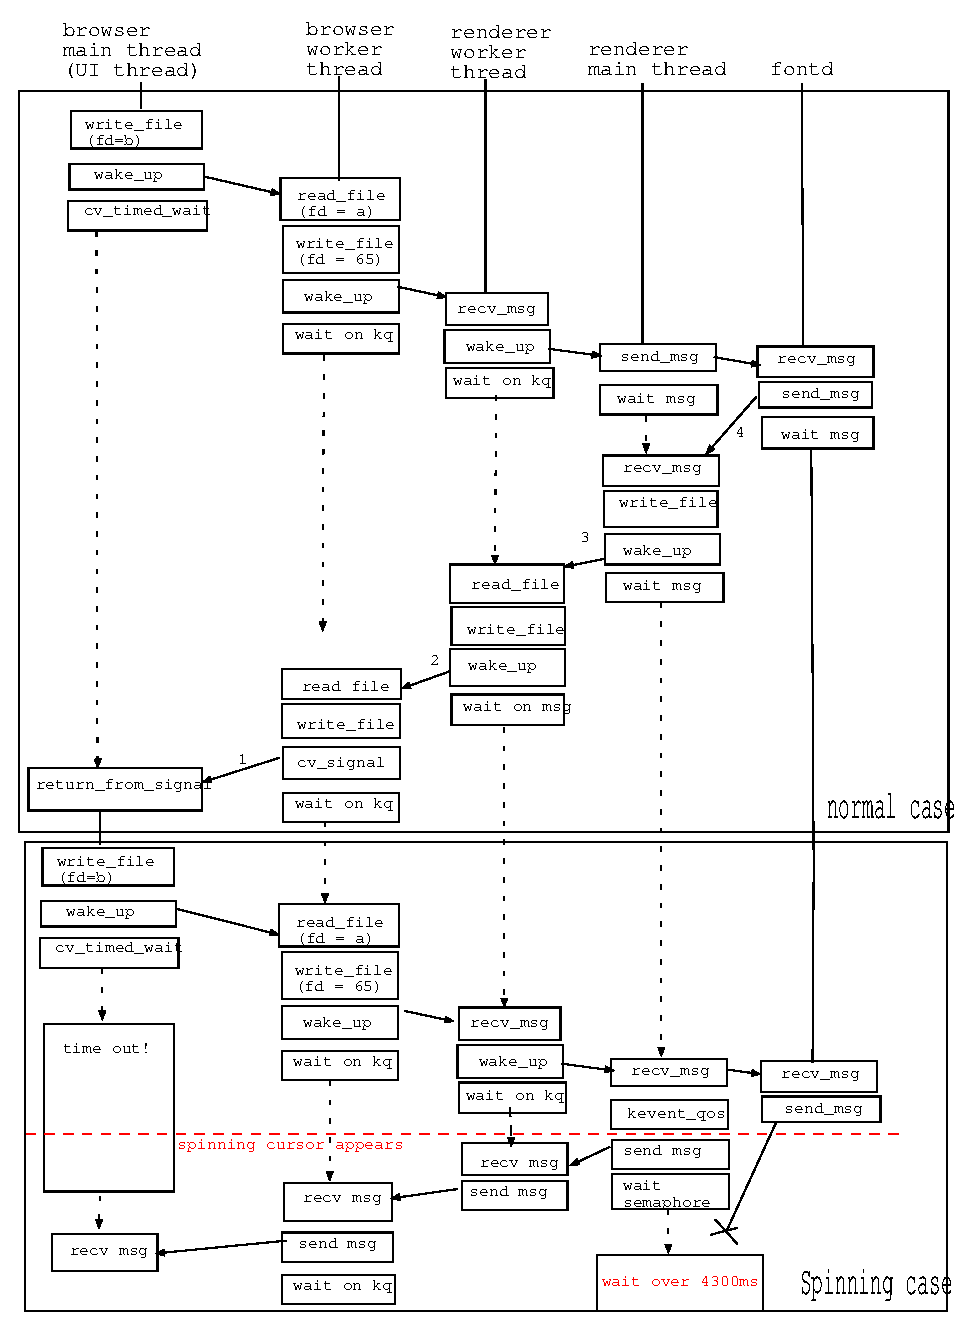
\includegraphics[width=1.0\linewidth]{chromium_case_study.eps}
    \caption{Chromium case study.}
    \label{fig:chromium-trace}
\end{figure}

\begin{figure}[tb]
    \centering
    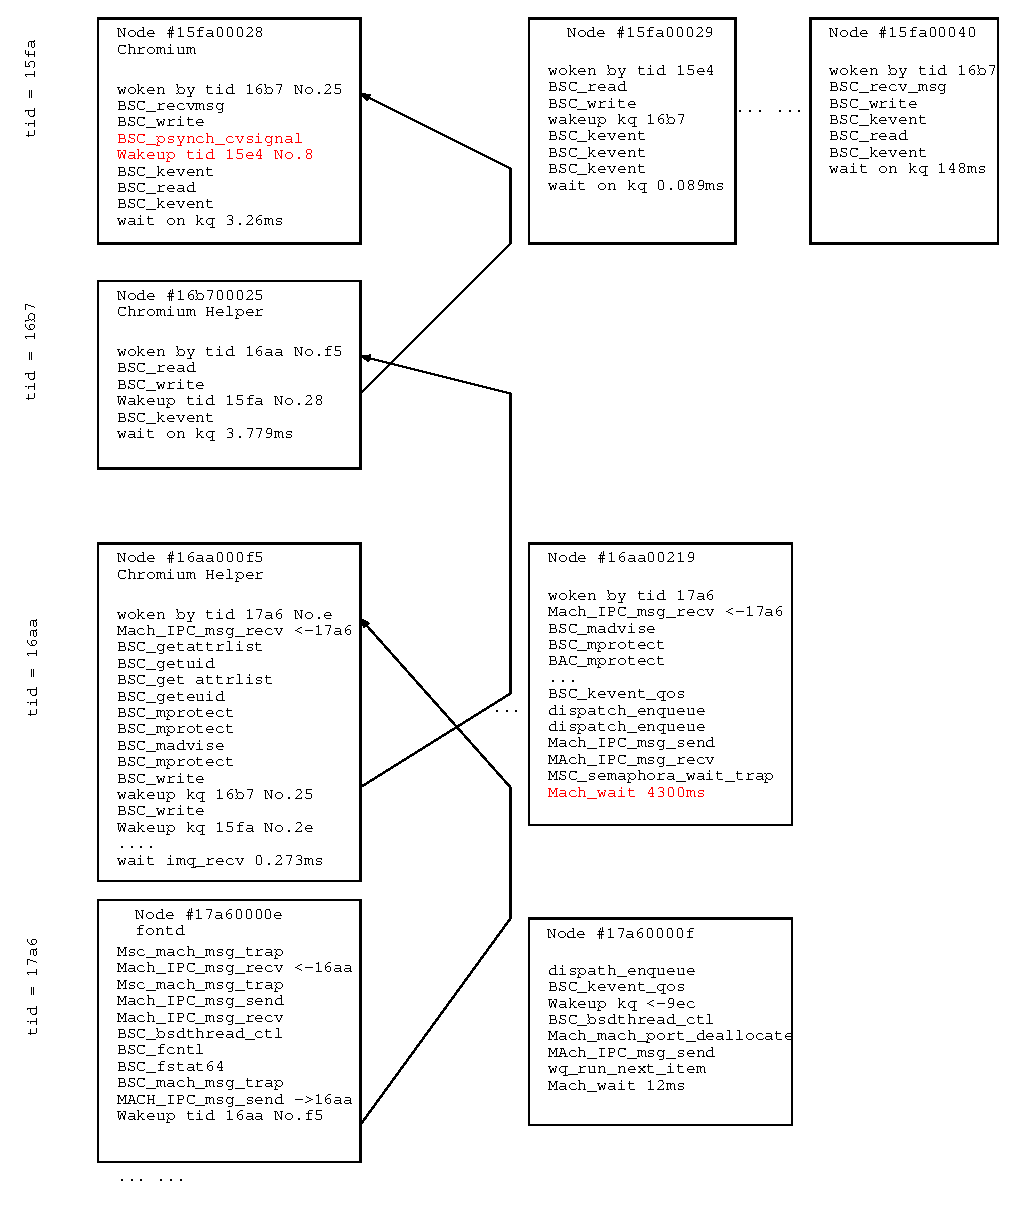
\includegraphics[width=1.0\linewidth]{backward_slicing_chromium.eps}
    \caption{Chromium backward path slicing.}
    \label{fig:path-slice-on-chromium}
\end{figure}

\subsection{chromium IME responsive}
One of the long lasting performance issue in chromium is hanging caused by the non-English input.
When users try to type non English to textFields, such as search box,
the main thread of the browser becomes non responsive.
With lldb it is not hard to tell that the main thread get stuck on FindFirstRect,
where the main thread waits for the signal of condition variable.
According to the history in bug report, the developers realized there were deadlocks somewhere.
However, it was hard to pinpoint due to the multiprocess and multithread programing paradigms.
As a result, timeout was added to prevent the deadlock, but not the long latency.
Although a further bug patch introducing cache helps to eliminate the long hanging mostly, 
the performance issue still appears from time to time.
The senario we can reproduce is to open the website of yahoo and quickly type Simplified Chinese.

The ground true we reveal with out tool is as shown in the picture XXX.
In chromium, there are one browser process and multiple renderer processes.
The main thread of the browser process try to get the caret position.
It sends out the message and wait for the reply on a condition variable.
Usually, a worker thread in the browser process will return the firstrect and wake up the main thread.
Howeve, it requires the message from the main thread of a renderer process to proceed.
Without the message from the renderer process, the worker thread is not able to signal the main thread,
thus, the main thread in will always time out.

Our trace tool will collect the data system wide, therefore, all the thread relationships are captured.
With the trace log size, both the hanging case and non-hanging case are recorded.
From the shared condition variable between threads, we are able to align the logs of the two cases,
and discover the missing message in the hanging case.

As we known the unresponsive of the main thread in the renderer process,
we further consult the analyzed trace log and observe that it is waiting on a semaphre,
and eventually waken by the main thread of the browser process.

Our tool further reveal the root cause of the livelock with conditional debugging.
We can either binary instrument or modify the source code to make the renderer thread accept the attachment of lldb.
The concrete call stacks from lldb disclose the task processing in the renderer thread is related to running javascript.

\subsubsection{System Preferences}

System Preferences provides a central location in macOS to customize system
settings. The ``Display'' pane allows users to configure additional monitors,
mirroring or extending their work space. However, the software does not support
disabling monitors that are online (the user must physically unplug monitors).
There is a tool called DisableMonitor~\cite{disablemonitor}, distributed via
GitHub, which addresses this functionality. Surprisingly, we find performance
bug in System Preferences when we disable an external monitor, and rearrange
the windows in the Display panel afterward. The System Preferences windows
freezes for seconds in this situation.

To diagnose this issue, we run the System Preferences app with \xxx. We
rearrange the displays with two active monitors, and repeat the process with
one of them deactivated. \xxx collects 132MB data, and constructs dependency
graph system-wide in the period, which contains 428,785 vertexes and 320,554
edges.

To diagnose the root cause, \xxx first finds out when the NSEvent thread in
System Preferences notifies WindowServer to draw the spinning cursor and marks
it as \textit{t}. The node in the main UI thread causing the non-responsiveness
must overlap the time interval \textit{(t - 2s, t)}. It is not hard for
\xxx to tell the spinning node in the main UI thread, either busy processing or
blocking.

The spinning node in the main UI thread is dominated by \textit{mach\_msg} and
\textit{thread\_switch}, both of which are meant to wait for available data
ping from WindowServer. Noticing the timeouts of \text{thread\_switch}, \xxx
classifies this case into the third category (\S\ref{subsec:debug}) and heads
to find a comparable normal node in the same thread. As its semantics are not
descriptive enough to identify its comparable node, \xxx extends the comparison
with its proceeding nodes.

In the normal case, System Preferences gets rid of the thread\_switch
quickly after receiving messages from WindowServer. It proceeds
to \textit{displayReconfigured}. On the other hand, the spinning
node ends up sending message for the available datagram ping with
\textit{CGSSnarfAndDispatchDatagrams}. By checking the lightweight call stacks,
\xxx figures out the messages from WindowServer in the previous nodes are
responses to data available pings from \textit{activeDisplayNotificationHandler}.

Given the information, we launched the interactive debugging by 
feeding the debugging script with those APIs mentioned above. We set the method
\textit{activeDisplayNotificationHandler} as a breakpoint where the script begins
debugging. \textit{displayReconfigured} and \textit{CGSSnarfAndDispatchDatagrams}
are used to indicate the end of debugging for the normal case and spinning case
respectively.

By diffing the two logs, we notice the different
branches in \textit{display\_notify\_proc} called by
\textit{activeDisplayNotificationHandler}. The handler depends on received
datagram and two shared variables ``\vv{\_gCGWillReconfigureSeen}'' and
``\vv{\_gCGDidReconfigureSeen}'' to finish a display configuration. In
both case the first variable is set to indicate the begin of display
configuration. In normal case, it receives a datagram which set the variable
``\vv{\_gCGDidReconfigureSeen}'' in \textit{display\_notify\_proc} and
finish display reconfiguration, while in the spinning case such datagram
is never received. Instead, an alternative datagram just drive it through
\textit{display\_notify\_proc} without setting any variable, which causes the
repeating \textit{thread\_switch} in the handler.

[In conclusion, the bug is... would have to be fixed by... we provide a binary fix...]


\section{Evaluation}
We first presents the results from the live deployment of Argus.
We demonstrate the overhead of our tracing tool intruduced, regarding the storage, memory and CPU usage.
Then we list the softwares which trigger spinning wait cursors in MacOs and the root cause we figure out with our framework.
At the end, we summaries the tedious work that our tool can take over from the user and make the diagnosis much easier in the wild.

\begin{itemize}
\item tracing overhead
	\begin{itemize}
	\item memory and CPU usage on top, while running ibench with and without our tracing enabled
	\item memory and CPU usage on top, while running the listed real world applications with and without our tracing enabled
	\item how much times it takes to filled the buffer we fixed 2G
	\item how many events recorded in the buffer
	\end{itemize}
\item number of edges and nodes in the graphs and portions of data the user need to examine to figure out the root cause.
\end{itemize}

\input{discussion}
\section{Related Work}

While there is currently no system that can help users debug performance
issues in closed-source applications on proprietary MacOS, several active
research topics are closely related.

\textbf{Event tracing.}  Magpie~\cite{magpie} is perhaps the closest to
our work.  It monitors server applications in Windows with the goal to
model the normal behaviors of a server application in response to a
workload.  This model further helps detecting anomalies statistically.  In
contrast, \xxx's goal is to identify the root causes of performance
issues.  Its graphs are not request graphs, but rather graphs that may
contain many requests.  In addition, it logs normal and abnormal
executions in the same event trace.  In addition, Magpie requires a
manual-written event schema for all involved applications to capture
precise request graphs, whereas \xxx has a simple, application-agnostic
schema for system-wide tracing and enables users to provide more
application-specific knowledge on demand.

Panappticon \cite{pannappticon} monitors a mobile system and uses the
trace to characterize the user transactions of mobile apps.  Although it
aims to track system-wide events and correlate them without developer
input, it supports only two models of communication: work queue and thread
pooling.

AppInsight \cite{appinsight} instruments application to identify the
critical execution path in a user transaction.  It supports the event
callback pattern, and does not trace across process or app boundaries.
                                                                                                                         
XTrace and Pinpoint \cite{xtrace, pinpoint} both trace the path of a
request through a system using a unique identifier attached to each
request and stitch traces together with the identifier.  \xxx does not
assume the presence of a unified identifier in closed-source, third-party
applications, frameworks, and libraries.
                                                                                                                         
Aguilela \cite{blackbox} uses timing analysis to correlate messages to
recover their input-output relations while treating the application as a
black box.

\textbf{Performance anomaly detection.}  Several systems detect
performance anomalies automatically.  \cite{} leverage the user logs and
call stacks to identify the performance anomaly. \cite{} apply the machine
learning method to identify the unusual event sequence as an anomaly.
\cite{} generates the wait and waken graph from sampled call stacks to
stidy a case of performance anomaly.  These systems are orthogonal to \xxx
as \xxx's goal is to diagnose an already-detected performance anomaly.
These systems can help \xxx by detecting more accurately when a
performance issue arises.

\section{Conclusion} \label{sec:conclusion}

Our key insight in this paper is that causal tracing is inherently inaccurate.
Those inaccuracy are unlikly remidied with heuristics to generate an request
graph feasible to automate diagnosis of performance issues. We built \xxx, a
practical system for effectively debugging performance issues despite inaccurate
causal tracing. It lets a user provide domain knowledge interactively on demand
to mitigate the inaccuracy. Compared to all upfront knowledge, this method is
more general and efficient given the various programing paradigms.

%Our results show that \xxx effectively
%helped us locate all root causes of the issues, including a bug in Chromium,
%01 and incurred \cpuoverhead CPU overhead overall in its system-wide tracing.
\clearpage


\bibliographystyle{plain}
\bibliography{bib/biblio}

\end{document}

